% exercise sheet with header on every page for math or close subjects
\documentclass[12pt]{article}
\usepackage[utf8]{inputenc}
\usepackage{latexsym}
\usepackage{multicol}
\usepackage{fancyhdr}
\usepackage{amsfonts}
\usepackage{amsmath}
\usepackage{amssymb}
\usepackage{enumerate}
\usepackage{listings}
\usepackage{graphicx}
\usepackage{pifont}

% Shortcuts for bb, frak and cal letters
\newcommand{\E}{\mathbb{E}}
\newcommand{\V}{\mathbb{V}}
\renewcommand{\P}{\mathbb{P}}
\newcommand{\N}{\mathbb{N}}
\newcommand{\R}{\mathbb{R}}
\newcommand{\C}{\mathbb{C}}
\newcommand{\Z}{\mathbb{Z}}
\newcommand{\Pfrak}{\mathfrak{P}}
\newcommand{\Pfrac}{\mathfrak{P}}
\newcommand{\Bfrac}{\mathfrak{P}}
\newcommand{\Bfrak}{\mathfrak{B}}
\newcommand{\Fcal}{\mathcal{F}}
\newcommand{\Ycal}{\mathcal{Y}}
\newcommand{\Bcal}{\mathcal{B}}
\newcommand{\Acal}{\mathcal{A}}

% formating
\topmargin -3.5cm
\textheight 22cm
\textwidth 16.0 cm
\oddsidemargin -0.1cm

% Fancy Header on every Page
\pagestyle{fancy}
\lhead{\textbf{Embedded Systems Problem Set G}}
\rhead{Rafael Dewes (2548365) \\ Kevin M\"uller (2550062) \\ Daniel Schäfer (2549458) }
\renewcommand{\headrulewidth}{1.2pt}
\setlength{\headheight}{110pt}

\begin{document}
\pagenumbering{gobble}
\lstset{language=C++}


\section*{Problem G1: Reactive Synthesis}
%TODO
\subsection*{a)}
From time to time, she realizes that she is late:
\[ \mathbf{GF} \: realize\_late \]
She will eventually start speeding, but never twice in a row:
\[ (\mathbf{F} \: speeding) \land \mathbf{G}(speeding \rightarrow \mathbf{X} \neg speeding) \]
When speeding in front of a police car, she has to go to jail some time in the future:
\[ \mathbf{G}(speeding \land near\_police\_car) \rightarrow (\mathbf{F} \: in\_jail) \]

We get the complete requirements by conjoining the above:
\[ (\mathbf{GF} \: r) \land ((\mathbf{F} \: s) \land \mathbf{G}(s \rightarrow \mathbf{X} \neg s)) \land (\mathbf{G}(s \land p) \rightarrow (\mathbf{F} \: j)) \]

\section*{Problem G2: Timed Synthesis}
\subsection*{a)}
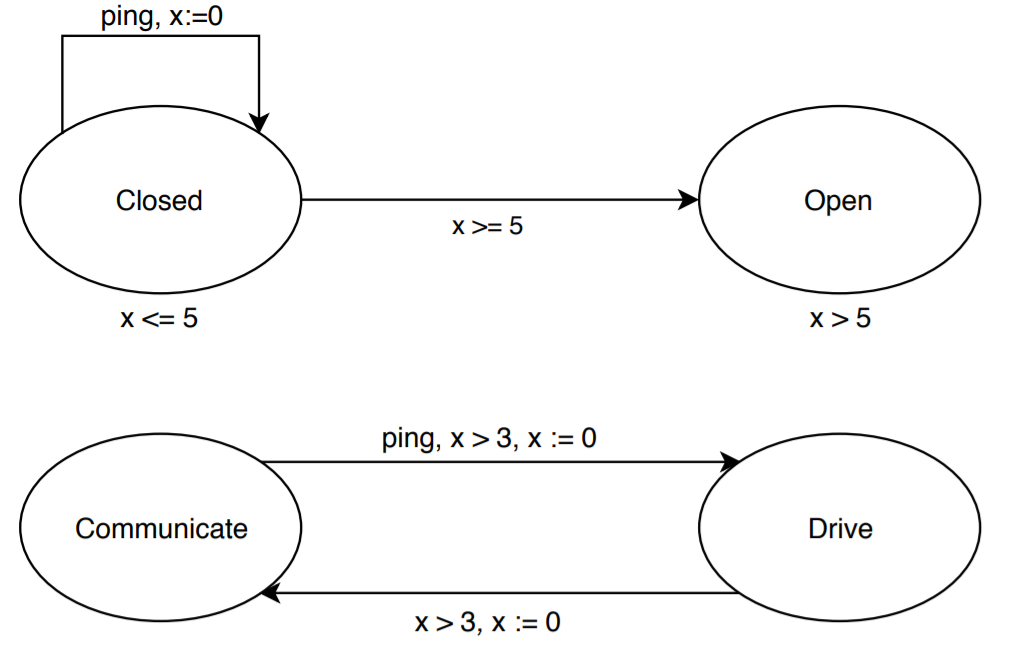
\includegraphics[width=0.8\textwidth]{TA.png}

\subsection*{b)}
The train can switch modes every three seconds. A ping is send on a mode switch from communication to drive. The gate will open once it does not receive a ping for 5 seconds. This means that the train will be able to send one ping but has to wait for 6 seconds before it can send the next ping. By that time, the gate will have openend. Therfore, there is no winning strategy for the train.

\section*{Problem G3: Parity Games}
%TODO

\paragraph*{Player 0 wins from every state:}
\[ \: \]
We can see that in every infinite play, the color 4 will be seen infinitely often. From states 1 and 3, Player 0 will always go back to 4. Also Player 0 can (and should) always prevent a game from going through the 5 in the middle. Therefore, any $x$ and $y < 5$ will be winning plays for Player 0 from every state because the highest color will be 4 which is even. \\
For $x = 5 \land y \leq 5$, Player 0 cannot prevent plays from going through 5 because from the upper 4, Player 1 can go to $x=5$ and from the lower 4, Player 0 will go to $y$ from where Player 0 either has to go to the 5 in the middle or to the upper 4 from where Player 1 will again choose to go to $x=5$. In any case, $x=5$ will be visited infinitely often. Again, Player 0 will win from every state. The same holds for $y = 5 \land x \leq 5$. \\
The winning valuations of $x$ and $y$ are indicated with an \checkmark \\
\\
\begin{tabular}{c | c | c | c | c | c | c}
$_y ^x$ & $\:$0$\:$ & $\:$1$\:$ & $\:$2$\:$ & $\:$3$\:$ & $\:$4$\:$ & $\:$5$\:$ \\ \hline
0 & \checkmark & \checkmark & \checkmark & \checkmark & \checkmark & x \\ \hline
1 & \checkmark & \checkmark & \checkmark & \checkmark & \checkmark & x \\ \hline
2 & \checkmark & \checkmark & \checkmark & \checkmark & \checkmark & x \\ \hline
3 & \checkmark & \checkmark & \checkmark & \checkmark & \checkmark & x \\ \hline
4 & \checkmark & \checkmark & \checkmark & \checkmark & \checkmark & x \\ \hline
5 & x & x & x & x & x & x \\ 


\end{tabular}

\paragraph*{Player 1 wins from every state:}
\[ \: \]
Obviously, valuation of $x$ and $y$ where Player 0 wins from every state, Player 1 cannot also win from every state. Therefore for every $x < 5 \land y < 5$ Player 1 cannot win from every state. The question remains whether Player 1 can win from $x < 5 \lor y < 5$. In fact this is the case because Player 0 cannot prevent the play from going into one of the states with color 4 as explained above.\\
So, for every valuation of $x$ and $y$ one of the players wins from every state.
The table for valuations where Player 1 wins from every state is the inverted table from above.\\
\\
\begin{tabular}{c | c | c | c | c | c | c}
$_y ^x$ & $\:$0$\:$ & $\:$1$\:$ & $\:$2$\:$ & $\:$3$\:$ & $\:$4$\:$ & $\:$5$\:$ \\ \hline
0 & x & x & x & x & x & \checkmark \\ \hline
1 & x & x & x & x & x & \checkmark \\ \hline
2 & x & x & x & x & x & \checkmark \\ \hline
3 & x & x & x & x & x & \checkmark \\ \hline
4 & x & x & x & x & x & \checkmark \\ \hline
5 & \checkmark & \checkmark & \checkmark & \checkmark & \checkmark & \checkmark \\ 

\end{tabular}

\end{document}
